\documentclass[12pt, a4paper]{article}

\usepackage[utf8]{inputenc}
\usepackage{amsfonts, amsmath, amssymb, amsthm}
\usepackage{geometry}
\usepackage[hidelinks]{hyperref}
\usepackage[none]{hyphenat}
\usepackage{setspace}
\usepackage{float}
\usepackage{fancyhdr}
\usepackage{enumitem}
\usepackage{graphicx}
\usepackage{cleveref}
\usepackage{tikz}

\geometry{a4paper, left=1in, top=1in, right=1in, bottom=1in}
\onehalfspacing

\newtheorem{theorem}{Theorem}[section]
\newtheorem{lemma}{Lemma}[section]
\newtheorem{corollary}{Corollary}[theorem]
\theoremstyle{definition}
\newtheorem{definition}{Definition}[section]
\newtheorem{example}{Example}[section]
\theoremstyle{remark}
\newtheorem*{remark}{\textbf{Remark}}

\newcommand{\e}{\varepsilon}
\newcommand{\st}{\text{ such that }}

\hyphenpenalty=10000
\exhyphenpenalty=10000

\title{\textbf{\Large Geometric Applications of the Riemann Integral: \\ \large Bridging Physical Intuition and Mathematical Rigour}}
\author{\textbf{Tushar Kumar Aich} \\
\small{Department of Mathematics, Tinsukia College}
}

\begin{document}
\maketitle

\begin{abstract}
    In introductory calculus and physics, geometric quantities such as area, volume and arc length are often treated as intuitive axioms derived from "slicing". While physically good, these definitions lack analytical well-definedness without the Riemann Integral. This note provides a rigorous reconstruction of these quantities from first principles. We demonstrate that the volume of a solid of revolution is not merely a sum of disks, but a limit bounded by Upper and Lower Darboux sums. Then we examine the problem of rectifiability, showing that the standard arc length formula is not an immediate consequence of the distance formula, but explicitly requires the Mean Value Theorem to justify the transition from discrete polygon approximation to a continuous integral.
\end{abstract}

\section{Introduction}
Wlile the \textbf{Fundamental Theorem of Calculus} provides the computational power to evaluate integrals, it is the Riemann-Darboux construction that provides the rigorous definitions of geometric objects. Here, we examine the analytical foundations of three classic applications:
\begin{itemize}
    \item \textbf{The Area Between Curves:} We define the area of a region bounded by two functions, proving that the quantity is well-defined under vertical translation for an pair of integrable functions.
    \item \textbf{The Length of a Curve:} We define arc length as the supremum of the lengths of inscribed polygons and demonstrate that the transition to the integral formula explicitly requires the \textbf{Lagrange's Mean Value Theorem}.
    \item \textbf{The Volume of a Solid:} We construct the volume of a solid of revolution not merely as a sum of disks, but as a unique limit "squeezed" between the Lower and Upper Darboux sums of the squared function.
\end{itemize}

\section{The Area Between Curves}
If two functions $f$ and $g$ are related by the inequality $f(x) \le g(x)$ for all $x \in [a,b]$, we write $f \le g$ on $[a,b]$, the set $S$ consisting of all points $(x,y)$ satisfying the inequalities,
\[
f(x) \le y \le g(x), \qquad a \le x \le b
\]
is called the region between the graphs $f$ and $g$.

\begin{theorem}
    Assume $f$ and $g$ are integrable functions on $[a,b]$ such that $f(x) \le g(x)$ for all $x \in [a,b]$. Then the area $A$ of the region $S$ between their graphs is given by:
    \[
    A = \int_a^b [g(x) - f(x)]dx
    \]
\end{theorem}

\begin{proof}
    \begin{figure}[H]
        \centering
        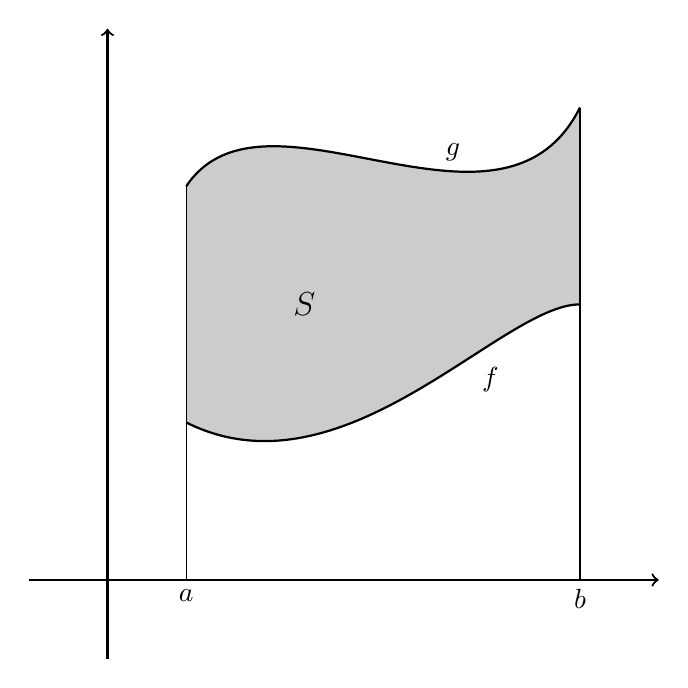
\begin{tikzpicture}
        %\draw[step=1cm,gray,very thin] (-2,-2) grid (6,6);

        \draw[thick, ->] (-2,-1) -- (6,-1);
        \draw[thick, ->] (-1,-2) -- (-1,6);

        \coordinate (f_start) at (0,1);
        \coordinate (f_end) at (5,2.5);
        \coordinate (g_start) at (0,4);
        \coordinate (g_end) at (5,5);

        \node[below] at (0,-1) {$a$};
        \node[below] at (5,-1) {$b$};

        \def\curveF{(f_start) .. controls (2,0) and (4,2.5) .. (f_end)}
        \def\curveG{(g_start) .. controls (1,5.5) and (4,3) .. (g_end)}
    
        \fill[gray!40] \curveF -- (g_end) .. controls (4,3) and (1,5.5) .. (g_start);

        \draw[thick] \curveF node[pos=0.65, below right] {$f$};
        \draw[thick] \curveG node[pos=0.65, above] {$g$};

        \draw (0,-1) -- (0,4);
        \draw (5,-1) -- (5,5);

        \node at (1.5, 2.5) {\large $S$};
        \end{tikzpicture}

        \caption{Non-negative functions}
        \label{fig:1}
    \end{figure}
    
    
    First, we consider the case $f$ and $g$ are non-negative, as shown in the ~\Cref{fig:1}. Let $G$ be the area under $g$ and $F$ be the area under $f$. The region S is the difference between these two areas:
    \begin{align*}
        A &= Area(G) - Area(F) \\
        &= \int_a^b g(x)dx - \int_a^b f(x)dx
    \end{align*}
    By the \textbf{Linearity of integrals}, we can combine this into a single integral:
    \[A = \int_a^b [g(x) - f(x)]dx\]

    \begin{figure}[H]
        \centering
        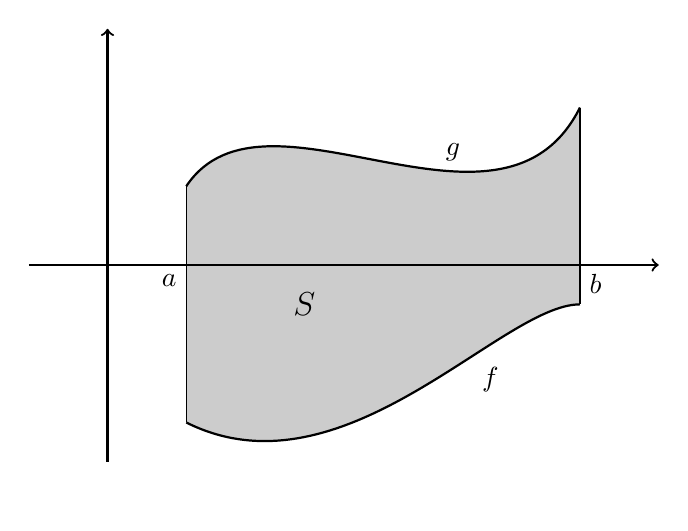
\begin{tikzpicture}
        %\draw[step=1cm,gray,very thin] (-2,-2) grid (6,6);

        \draw[thick, ->] (-1,0.5) -- (-1,6);

        \coordinate (f_start) at (0,1);
        \coordinate (f_end) at (5,2.5);
        \coordinate (g_start) at (0,4);
        \coordinate (g_end) at (5,5);

        \def\curveF{(f_start) .. controls (2,0) and (4,2.5) .. (f_end)}
        \def\curveG{(g_start) .. controls (1,5.5) and (4,3) .. (g_end)}
    
        \fill[gray!40] \curveF -- (g_end) .. controls (4,3) and (1,5.5) .. (g_start);

        \draw[thick] \curveF node[pos=0.65, below right] {$f$};
        \draw[thick] \curveG node[pos=0.65, above] {$g$};

        \draw (f_start) -- (g_start);
        \draw (f_end) -- (g_end);

        \draw[thick, ->] (-2,3) -- (6,3);

        \node[below left] at (0,3) {$a$};
        \node[below right] at (5,3) {$b$};

        \node at (1.5, 2.5) {\large $S$};
        \end{tikzpicture}
        \caption{General Case}
        \label{fig:2}
    \end{figure}
    Now, Consider the genral case where $f$ and $g$ are not necessarily non-negative, as shown in the ~\Cref{fig:2}. Because $f$ is Riemann integrable on $[a,b]$, it is bounded. Thus there exists a constant $C \in \mathbb{R}$ such that:
    \begin{align*}
        |f(x)| &\le C \qquad \text{for all } x \in [a,b]\\
        \implies -C \le f(x) &\le C
    \end{align*}
    Thus
    \[
    f(x)+C \ge 0 \qquad \text{for all } x \in [a,b]
    \]
    Since $g(x) \ge f(x)$, it follows that $g(x)+C \ge 0$ as well. Let us define a new region $T$ bounded by the shifted functions $g(x) + C$ and $f(x)+C$. Because a vertical shift is a rigid transformation, the area remains unchanged. Applying the result from the first case:
    \begin{align*}
        Area(T) &= \int_a^b [(g(x) + C) - (f(x) + C)] dx\\
        &= \int_a^b [g(x) + C - f(x) - C] dx\\
        &= \int_a^b [g(x) - f(x)]dx
    \end{align*}
    Since the area of the original region $S$ is equal to the area of the shifted region $T$, we conclude:
    \[
    A = \int_a^b [g(x) - f(x)]dx
    \]
\end{proof}

\begin{remark}
    It is important to note that this area formula holds true regardless of whether the functions lie above or below the x-axis. Because a vertical shift is a rigid transformation, shifting both functions upwards by a constant C to make them non-negative leaves the total area completely unchanged. The constant simply cancels out during the subtraction of the two functions.
\end{remark}

\section{The Length of a Curve}
Two different types of geometrical properties or quantities are associated with curves. The first type depends only on the behaviour of the curve in the small, that is, in the immediate neighborhood of a point; such properties are those which can be expressed by means of derivatives of a point. Properties of the second type or properties in the large depend on the whole configuration of the curve, and are usually expressed analytically by means of the concept of integral.

\begin{theorem}
    Assume $f$ is integrable on $[a,b]$. Also $f'(x)$ exists and is continuous for all $x \in [a,b]$. Then the length of the curve $S$ is given by:
    \[S = \int_a^b \sqrt{1+[f'(x)]^2} \ dx\]
\end{theorem}

\begin{proof}
    Let there be a partition $P$ of the interval $[a,b]$ such that:
    \[
    P = \{x_0, x_1, \ldots, x_n\} \quad \text{where } a=x_0 < x_1 < \ldots < x_n = b
    \]

    \begin{figure}
        \centering
        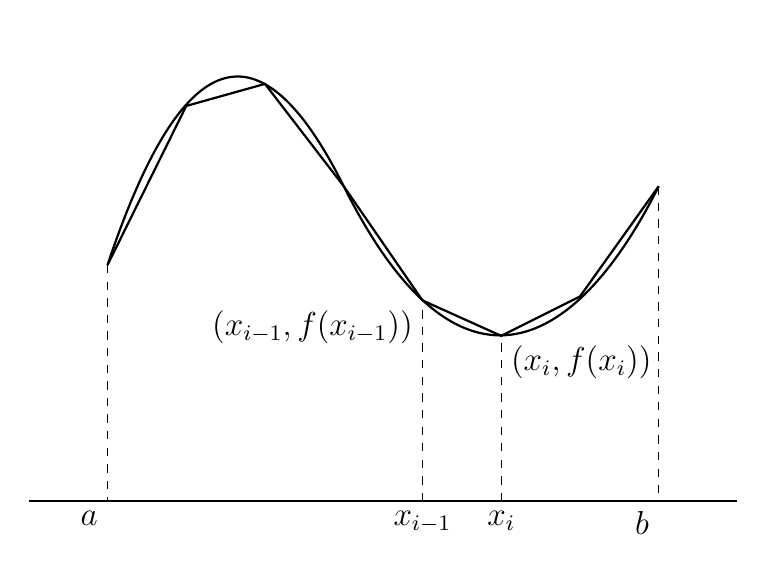
\begin{tikzpicture}
            %\draw[step=1cm,gray,very thin] (-2,-2) grid (7,5);

            \draw[thick] (-2,-1) -- (7,-1);
            %\draw[thick, ->] (-1,-2) -- (-1,6);

            \draw[thick] (-1,2) .. controls (0,5) and (1,5) .. (2,3) .. controls (3.5,0) and (5,1) .. (6,3);

            \draw[thick] (-1,2) -- (0,4.02) -- (1,4.3) -- (2,3) -- (3,1.55) -- (4,1.1) -- (5,1.6) -- (6,3);

            \draw[dashed] (-1,2) -- (-1,-1);
            \node[below left] at (-1,-1) (a) {\large$a$};

            \draw[dashed] (6,3) -- (6,-1);
            \node[below left] at (6,-1) (b) {\large$b$};

            \draw[dashed] (3,-1) -- (3,1.55);
            \node[below] at (3,-1) (x1) {\large$x_{i-1}$};
            \node[below left] at (3,1.55) (fx1) {\large$(x_{i-1}, f(x_{i-1}))$};

            \draw[dashed] (4,-1) -- (4,1.1);
            \node[below] at (4,-1) (x2) {\large$x_{i}$};
            \node[below right] at (4,1.1) (fx2) {\large$(x_{i}, f(x_{i}))$};
        \end{tikzpicture}
        \caption{Curve length approximation}
        \label{fig:3}
    \end{figure}
    By joining the points $x_{i-1}, f(x_{i-1})$ and $x_i, f(x_i)$, we form an inscribed polygon, as shown in ~\Cref{fig:3}. The total length S of the curve is approximated by the sum of the lengths of these line segments.

    Let $\Delta x_i = x_i - x_{i-1}$ and $\Delta y_i = f(x_i) - f(x_{i-1})$. The length of the line segment connecting these two points is given by the distance formula:
    \begin{equation}
        L_i = \sqrt{(x_i - x_{i-1})^2 + (f(x_i) - f(x_{i-1}))^2} = \sqrt{(\Delta x_i)^2 + (\Delta y_i)^2}
    \end{equation}
    Thus, the total length of the inscribed polygon, denoted as $S_n$, is the sum of these segments:
    \begin{equation}
        S_n = \sum_{i=1}^n L_i = \sum_{i=1}^n \sqrt{(\Delta x_i)^2 + (\Delta y_i)^2}
    \end{equation}
    Since $f$ is continuous on $[x_{i-1}, x_i]$ and differentiable on $(x_{i-1}, x_i)$, by the \textbf{Lagrange's Mean Value Theorem}, there exists a point $c_i \in (x_{i-1}, x_i)$ such that:
    \begin{align*}
        f'(c_i) &= \frac{f(x_i) - f(x_{i-1})}{x_i - x_{i-1}}\\
        \implies \Delta y_i &= f'(c_i) \Delta x_i \tag{3}
    \end{align*}
    Now, substituting the value of $\Delta y_i$ from equation (3) into equation (2), we get:
    \begin{align*}
        S_n &= \sum_{i=1}^n \sqrt{(\Delta x_i)^2 + (f'(c_i) \Delta x_i)^2} \\
        &= \sum_{i=1}^n \sqrt{(\Delta x_i)^2 (1 + (f'(c_i))^2)} \\
        &= \sum_{i=1}^n \sqrt{1 + (f'(c_i))^2} \Delta x_i \tag{4}
    \end{align*}
    As we increase the number of points such that $n$ approaches $\infty$ and the width of the largest subinterval approaches $0$, the sum $S_n$ converges to the integral. Thus finally the equation (4) becomes:
    \[
    S = \int_a^b \sqrt{1 + [f'(x)]^2} \ dx
    \]
\end{proof}

\begin{remark}
    This theorem highlights a critical analytical bridge between discrete geometry and continuous calculus. While the length of the inscribed polygon relies purely on the standard algebraic distance formula, transitioning to the continuous integral formula explicitly requires Lagrange's Mean Value Theorem. It is this theorem that allows us to substitute the discrete vertical change with the continuous derivative $f^{\prime}(c_{i})$.
\end{remark}

\section{Volume of Revolving Curves}
\begin{theorem}
    Let $f$ be a continuous non-negative function on $[a,b]$. Then the volume $V$ of the solid obtained by revolving the region bounded by the graph of $f$, the x-axis and the vertical lines $x=a$ and $x=b$ about the x-axis is given by:
    \[
    V = \pi \int_a^b [f(x)]^2 \, dx
    \]
\end{theorem}

\begin{proof}
    Let $P$ be a partition of the interval $[a,b]$ such that:
    \[
    P = \{x_0, x_1, \ldots, x_n\} \quad \text{where } a=x_0 < x_1 < \ldots < x_n = b
    \]
    Let $\Delta x_i = x_i - x_{i-1}$ denote the $i$-th subinterval.

    Since $f$ is continuous on the interval $[x_{i-1}, x_i]$, thus by the \textbf{Extreme Value Theorem}, there exist points $m_i$ and $M_i$ in $[x_{i-1}, x_i]$ such that:
    \begin{align*}
        m_i = \inf {f(x) : x \in [x_{i-1}, x_i]} \\
        M_i = \sup {f(x) : x \in [x_{i-1}, x_i]}
    \end{align*}
    The solid slice $\Delta V_i$ generated over the subinterval $[x_{i-1}, x_i]$ is bounded by two cylinders: an inner cyliner of radius $m_i$ and an outer cylinder of radius $M_i$. Thus, the volume of the solid slice satisfies the inequality:
    \[
    \pi (m_i)^2 \Delta x_i \le \Delta V_i \le \pi (M_i)^2 \Delta x_i
    \]
    Summing the inequality all over all $n$ subintervals from $i=1$ to $n$, we obtain bounds for the total volume $V$:
    \[
    \sum_{i = 1}^{n} \pi (m_i)^2 \Delta x_i \le \sum_{i = 1}^{n} \Delta V_i \le \sum_{i = 1}^{n} \pi (M_i)^2 \Delta x_i
    \]

    Observing that $\sum \Delta V_i = V$, we can identify the terms on the left and right as the Lower and Upper Darboux sums for the function $g(x) = \pi f^2$ with respect to the partition $P$:
    \[
    L(\pi f^2, P) \le V \le U(\pi f^2, P)
    \]
    Since $f$ is continuous on $[a,b]$, the function $g(x) = \pi f^2$ is also continuous and hence integrable on $[a,b]$. This implies that the norm of partition approaches zero $(\|P\| \to 0)$, the Lower and Upper Darboux sums converge to the same limit, which is the integral of $g$:
    \[
    \lim_{\|P\| \to 0} L(\pi f^2, P) = \lim_{\|P\| \to 0} U(\pi f^2, P) = \int_a^b \pi [f(x)]^2 dx
    \]

    Since the volume $V$ is "trapped" between $L$ and $U$ for any partition $P$, it must be equal to the integral limit. Therefore, we conclude:
    \[
    V = \pi \int_a^b [f(x)]^2 \ dx
    \]
\end{proof}

\begin{remark}
    While introductory calculus often presents the volume of a solid of revolution intuitively as a simple "sum of disks," its rigorous justification requires bounding the solid. The true volume is analytically "trapped" between inner and outer cylindrical slices, representing the Lower and Upper Darboux sums of the function $g(x)=\pi f^{2}$. Because the function is continuous, these bounding sums are guaranteed to converge to a single, unique integral limit as the partition norm approaches zero.
\end{remark}

\newpage

\begin{thebibliography}{9}
    \bibitem{spivak}
    Spivak, M. (2008). \textit{Calculus} (4th ed.). Publish or Perish.
\end{thebibliography}
\end{document}